\documentclass[10pt,mathserif]{beamer}
\usetheme{Rochester}
\definecolor{this.blue}{RGB}{52,101,164}
\definecolor{this.red}{RGB}{204,0,0}
\definecolor{this.green}{RGB}{102,153,0}
\definecolor{this.orange}{RGB}{242,148,51}
\usecolortheme[RGB={52,101,164}]{structure}
\setbeamercolor{block title}{fg=this.blue}
\setbeamercolor{block title alerted}{fg=this.red}
\setbeamercolor{block title example}{fg=this.green}
\usepackage[]{hyperref}
\usepackage[brazil]{babel}
\usepackage{lmodern}
\usepackage{ctable}
\usepackage{amssymb,amsmath,amsfonts}
\usepackage{ifxetex,ifluatex}
\ifxetex
  \usepackage{fontspec,xltxtra,xunicode}
  \defaultfontfeatures{Mapping=tex-text,Scale=MatchLowercase}
\else
  \ifluatex
    \usepackage{fontspec}
    \defaultfontfeatures{Mapping=tex-text,Scale=MatchLowercase}
  \else
    \usepackage[utf8]{inputenc}
  \fi
\fi
% Comment these out if you don't want a slide with just the
% part/section/subsection/subsubsection title:
%\AtBeginPart{\frame{\partpage}}
%\AtBeginSection{\frame{\sectionpage}}
%\AtBeginSubsection{\frame{\subsectionpage}}
%\AtBeginSubsubsection{\frame{\subsubsectionpage}}
% new commands
\newcommand{\slidetitle}[1]{
	{\begin{center}\Huge{\textbf{\textcolor[RGB]{52,101,164}{#1}}}\end{center}}
}
\newcommand{\slidesubtitle}[1]{
	{\begin{center}\huge{\textbf{\textcolor[RGB]{51,51,51}{#1}}}\end{center}}
}
\setlength{\parindent}{0pt}
\setlength{\parskip}{6pt plus 2pt minus 1pt}
\setlength{\emergencystretch}{3em}  % prevent overfull lines
\setcounter{secnumdepth}{0}

\title{Onde o Software Livre pode te levar}
\subtitle{Uma viagem ao mundo livre}
\author{Átila Camurça\\camurca.home@gmail.com\\Darlildo Lima\\darlildo.cefetce@gmail.com}

\begin{document}
\begin{frame}
\titlepage
\end{frame}

\begin{frame}\frametitle{Sumário}
\tableofcontents
\end{frame}

\section{Introdução}

\begin{frame}\frametitle{Introdução}

Software livre além de tudo é conhecimento. Sendo assim, não somente ser
livre é ideal porque é de graça, mas também porque te dá a liberdade de
aprender como é feito.

Tendo isso em mente vamos aprender que contribuir com software livre nem
sempre é contribuir com código-fonte.

\end{frame}

\begin{frame}\frametitle{}

\slidetitle{Tradução de aplicativos livres}

\end{frame}

\section{Tradução}

\subsection{Tradução de aplicativos livres}

\begin{frame}\frametitle{Tradução de aplicativos livres}

\begin{quote}
Tudo começou ao assistirmos no ENSL - Encontro Nordestino de Software
Livre, em Natal, uma palestra sobre o software
\href{http://noosfero.org/}{Noosfero}, uma plataforma web para redes
sociais e de economia solidária. Um dos tópicos foi a tradução do
aplicativo. Ao saber como um aplicativo era traduzido fomos capazes de
perceber uma forma de contribuir sem ter muito conhecimento técnico.

\end{quote}
\textbf{Dica:} ao assistir uma palestra não vá com a intenção de
entender tudo. Ao invés disso tente absorver aquilo que lhe é
interessante. Isso te dá o pontapé inicial para novas descobertas.

\end{frame}

\begin{frame}\frametitle{Tradução de aplicativos livres}

Átila:

\begin{quote}
\ldots{} depois de contribuir com o LaTeXila e ver ele como software
oficial de LaTeX do GNOME me deixou muito orgulhoso.

\end{quote}
\end{frame}

\begin{frame}\frametitle{Tradução de aplicativos livres}

\begin{figure}
   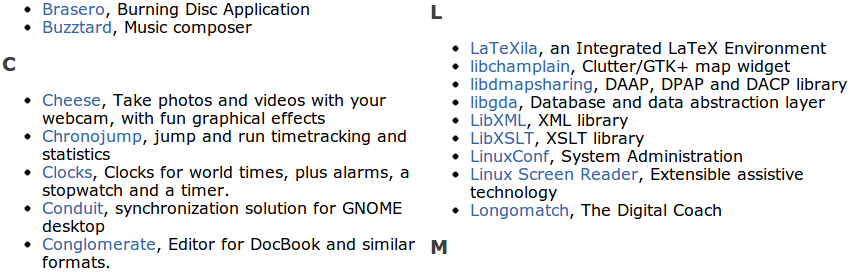
\includegraphics[scale=0.35]{img/latexila-1.png}
   \caption{LaTeXila em projects.gnome.org}
\end{figure}

\end{frame}

\begin{frame}[fragile]\frametitle{Tradução de aplicativos livres}

Entenda melhor o processo de tradução acessando o site

\url{http://www.mad3linux.org/p/downloads.html}

e procure pela palestra: Tradução de Aplicativos Livres.

\end{frame}

\begin{frame}\frametitle{}

\slidetitle{Tradução de documentos}

\end{frame}

\subsection{Tradução de documentos}

\begin{frame}[fragile]\frametitle{Tradução de documentos}

Com software livre tem a oportunidade de trabalhar com o pessoal do
Google, certo?

\begin{quote}
Com o HTML5 e CSS3 em alta, pesquisei sobre o assunto na internet. Achei
um site chamado \url{http://html5rocks.com} que continha vários slides
principalmente de desenvolvedores do Google. Decidi que no COMSOLiD 5
iria apresentar uma daquelas palestras. Achei o projeto dos slides, que
são web, e descobri que eram traduzíveis. Mais tarde, depois de traduzir
para apenas apresentar, decidi compartilhar as alterações. Acabou que o
Martin Gorner, desenvolvedor do Google, me adicionou como
\emph{commiter} e a apesentação de slides tem tradução para Português do
Brasil.

\end{quote}
\end{frame}

\begin{frame}\frametitle{Tradução de documentos}

\begin{figure}
   
\includegraphics[scale=0.35]{img/animateyourhtml5.png}
   \caption{animateyourhtml5.appspot.com}
\end{figure}

\end{frame}

\begin{frame}\frametitle{Tradução de documentos}

\begin{figure}
   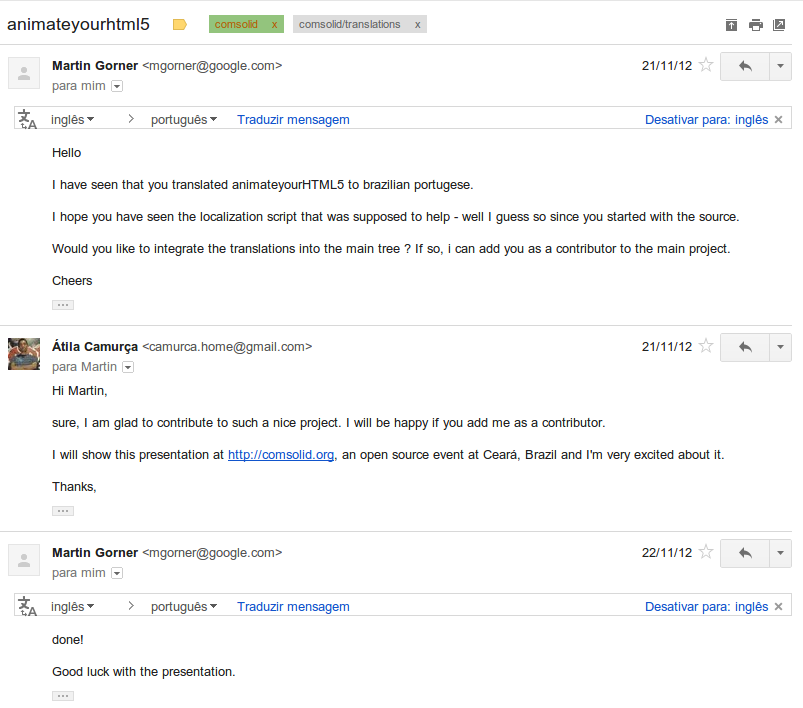
\includegraphics[scale=0.35]{img/martin-gorner.png}
\end{figure}

\end{frame}

\begin{frame}\frametitle{Tradução de documentos}

\begin{figure}
   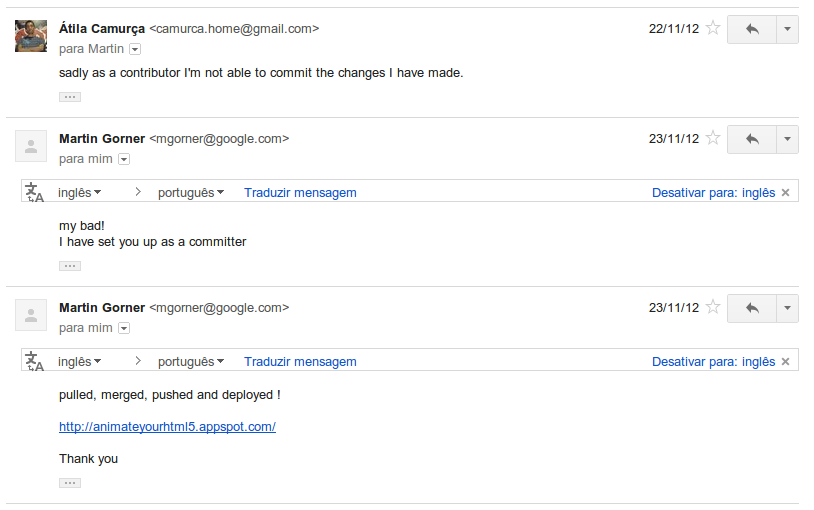
\includegraphics[scale=0.4]{img/martin-gorner-2.png}
\end{figure}

\end{frame}

\begin{frame}\frametitle{}

\slidetitle{Participação em eventos}

\end{frame}

\section{Participação em eventos}

\begin{frame}\frametitle{Participação em eventos}

Participar de eventos também é uma forma de contribuir, seja com relatos
sobre o que viu no evento, pessoas que conheceu, troca de ideias, enfim.

\end{frame}

\begin{frame}\frametitle{Participação em eventos}

\begin{figure}
   
\includegraphics[scale=0.25]{img/atilacamurca-comsolid5.jpg}
   \caption{COMSOLiD +5 2012}
\end{figure}

\end{frame}

\begin{frame}\frametitle{Participação em eventos}

\begin{figure}
   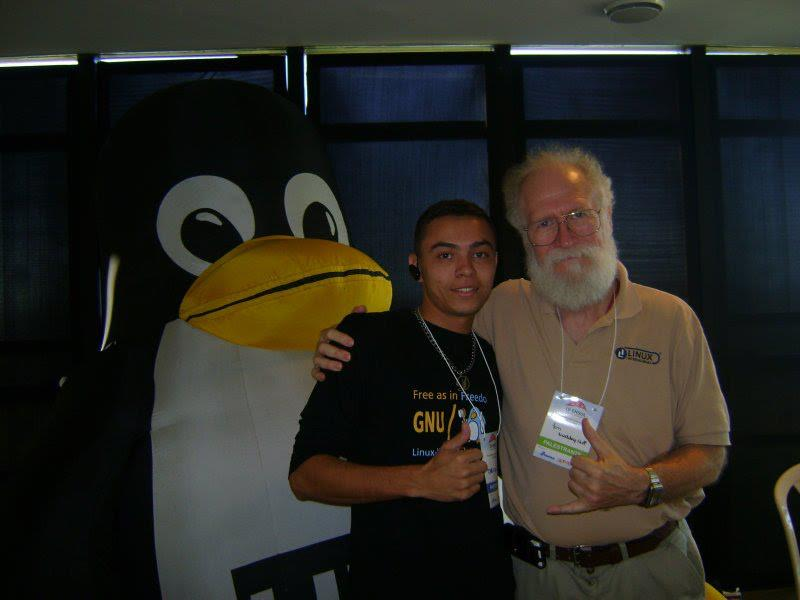
\includegraphics[scale=0.3]{img/darlildo-ensol2010.jpg}
   \caption{ENSOL 2010}
\end{figure}

\end{frame}

\begin{frame}\frametitle{Participação em eventos}

\begin{figure}
   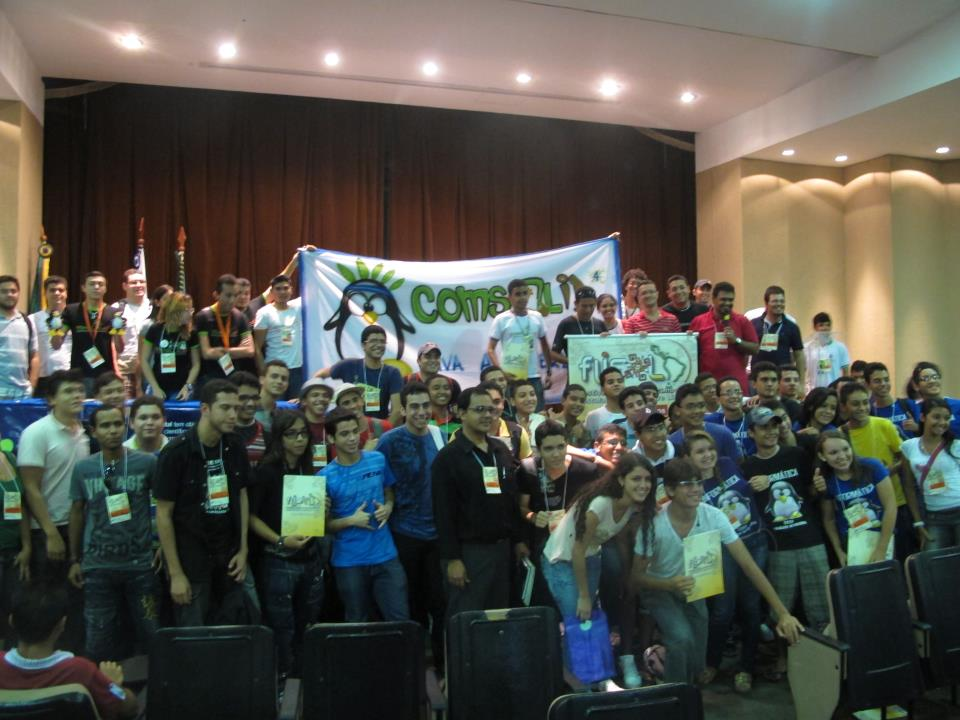
\includegraphics[scale=0.25]{img/atilacamurca-flisol-2012-3.jpg}
   \caption{FLISOL 2012}
\end{figure}

\end{frame}

\begin{frame}\frametitle{Participação em eventos}

\begin{figure}
   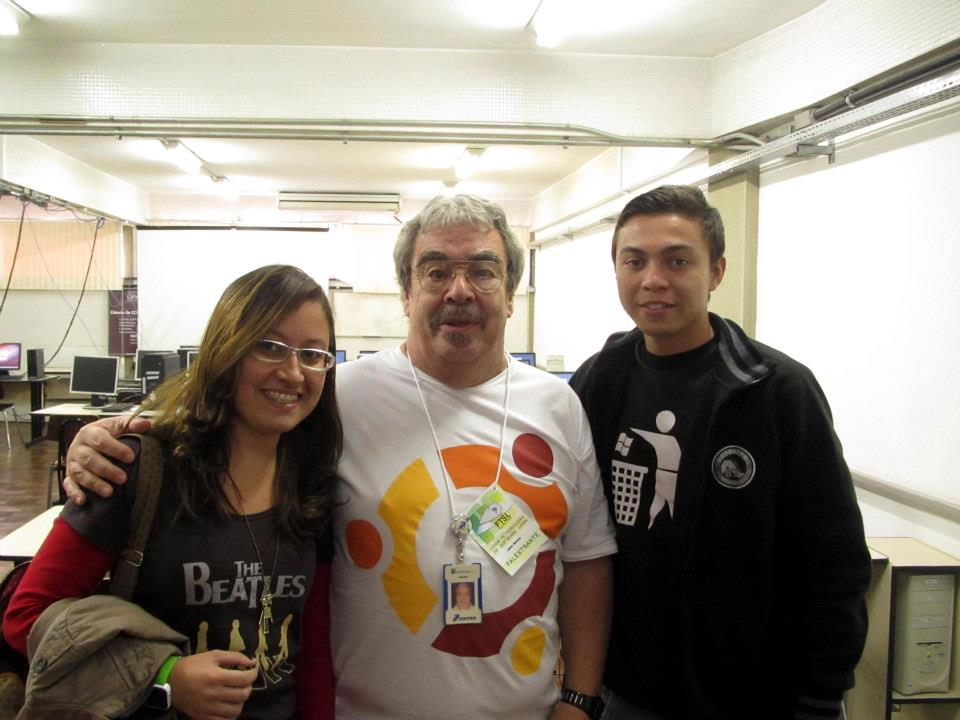
\includegraphics[scale=0.25]{img/darlildo-fisl-1.jpg}
   \caption{FISL 2012}
\end{figure}

\end{frame}

\begin{frame}\frametitle{Participação em eventos}

\begin{figure}
   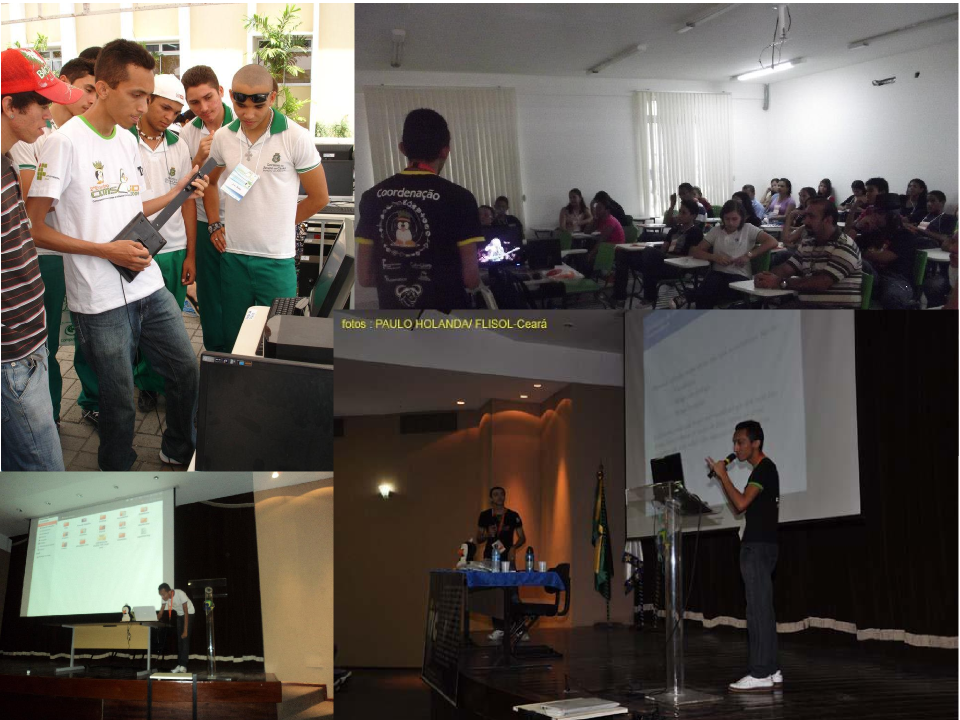
\includegraphics[scale=0.3]{img/wall-1.png}
\end{figure}

\end{frame}

\begin{frame}\frametitle{Participação em eventos}

\begin{figure}
   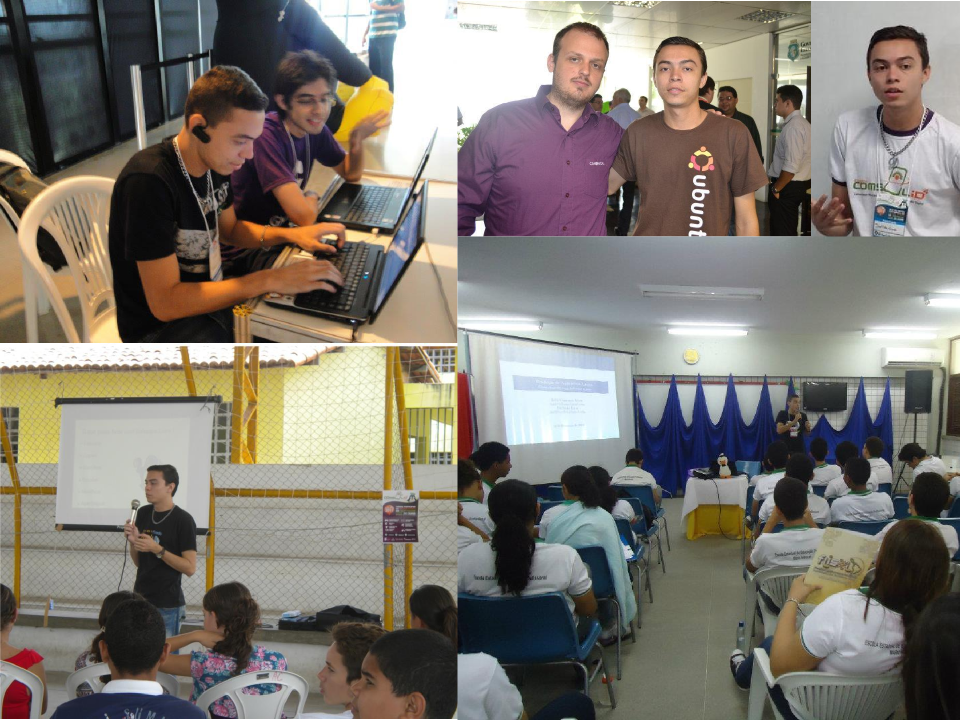
\includegraphics[scale=0.3]{img/wall-2.png}
\end{figure}

\end{frame}

\begin{frame}\frametitle{}

\slidetitle{Contribuição com código e conhecimento}

\end{frame}

\section{Contribuição com código e conhecimento}

\begin{frame}\frametitle{}

\slidesubtitle{github.com}

\begin{figure}
    
\includegraphics[scale=0.3]{img/github.jpg}
\end{figure}

\end{frame}

\begin{frame}[fragile]\frametitle{Contribuição com código e
conhecimento}

\url{http://github.com} - uma rede social de códigos-fonte.

Imaginem um local onde pessoas do mundo todo, programadores
profissionais, engenheiros, entre outros gênios da informática
disponibilizando códigos de todas as linguagens, onde é possível
contribuir de maneira fácil.

\end{frame}

\begin{frame}\frametitle{github.com}

Entre eles estão:

\begin{itemize}
\item
  \href{https://github.com/torvalds}{github.com/torvalds (Linus
  Torvalds)} - Criado do Linux e git
\item
  \href{https://github.com/fat}{github.com/fat} e
  \href{https://github.com/mdo}{github.com/mdo} - Criadores do Twitter
  Bootstrap
\item
  \href{https://github.com/jeresig}{github.com/jeresig} - Criador do
  jQuery
\item
  \href{https://github.com/rlerdorf}{github.com/rlerdorf} - Criador do
  PHP
\end{itemize}
\end{frame}

\begin{frame}\frametitle{github.com}

Além de empresas como:

\begin{columns}

    \begin{column}{4cm}
        \begin{figure}
            
\includegraphics[scale=0.2]{img/twitter.png}
            \caption{github.com/twitter}
        \end{figure}

        \begin{figure}
            
\includegraphics[scale=0.1]{img/facebook.jpg}
            \caption{github.com/facebook}
        \end{figure}
    \end{column}

    \begin{column}{4.5cm}
        \begin{figure}
            
\includegraphics[scale=0.2]{img/zend2.png} 
            \caption{github.com/zendframework}
        \end{figure}
        \begin{figure}
            
\includegraphics[scale=0.15]{img/wordpress.png} 
            \caption{github.com/WordPress}
        \end{figure}
    \end{column}

\end{columns}

\end{frame}

\begin{frame}\frametitle{github.com/atilacamurca}

\framesubtitle{github.com}

\begin{figure}
    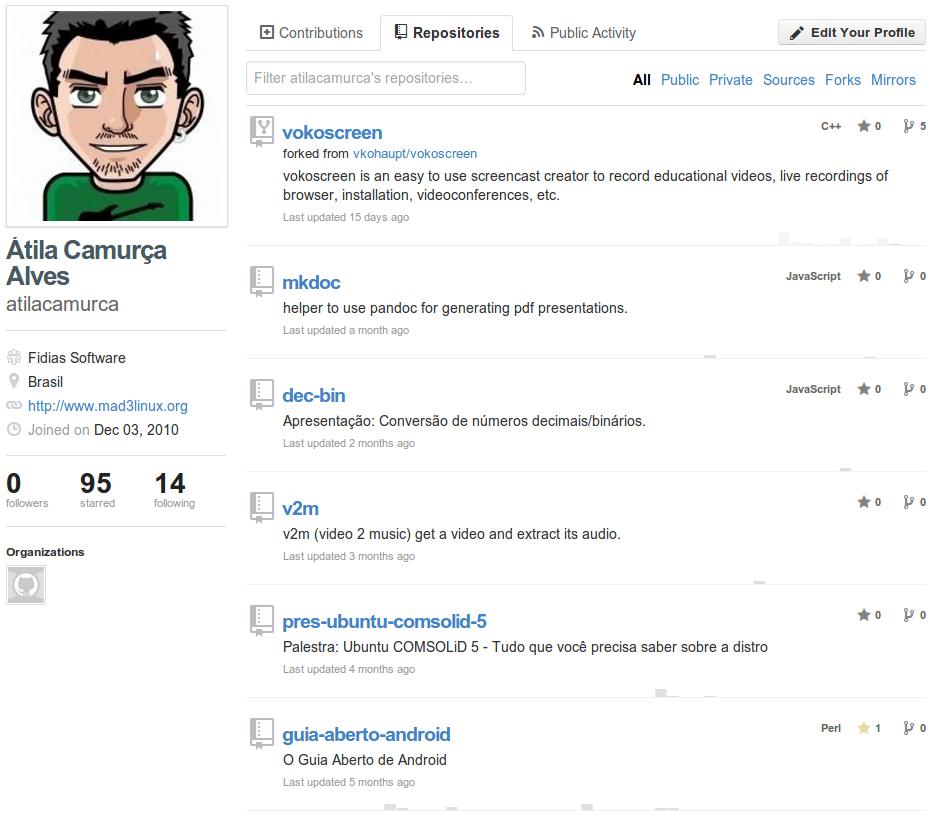
\includegraphics[scale=0.25]{img/github-atilacamurca.png}
\end{figure}

\end{frame}


\end{document}
